% Created 2018-03-13 火 09:33
\documentclass[11pt]{article}
\usepackage[utf8]{inputenc}
\usepackage[T1]{fontenc}
\usepackage{fixltx2e}
\usepackage{graphicx}
\usepackage{grffile}
\usepackage{longtable}
\usepackage{wrapfig}
\usepackage{rotating}
\usepackage[normalem]{ulem}
\usepackage{amsmath}
\usepackage{textcomp}
\usepackage{amssymb}
\usepackage{capt-of}
\usepackage{hyperref}
\author{Takehide Soh}
\date{\today}
\title{Introduction of Scala Programming Language  List and its Manipulation}
\begin{document}

\maketitle
\setcounter{tocdepth}{1}
\tableofcontents


\section{Overview}
\label{sec:orgheadline1}
\begin{quote}
The goal of this subject is to study the parser combinator of Scala
and the development of a calculator. 
\end{quote}

\section{Regular Expressions}
\label{sec:orgheadline3}
\begin{itemize}
\item of Scala is used to check that a
string is matched to a given pattern.
\item Note that, regular expressions correspond to  in
, that is, .

\item Reference (Wikipedia):
\begin{itemize}
\item \href{https://en.wikipedia.org/wiki/Regular_expression}{Regular Expression}
\item \href{https://en.wikipedia.org/wiki/Regular_language}{Regular Language}
\item \href{https://en.wikipedia.org/wiki/Formal_language}{Formal Language Theory}
\end{itemize}
\end{itemize}

For instance, a regular expression \texttt{w*} (asterisk) represent a pattern that 
iterates a character \texttt{w} \(n\) times (\(n \ge 0\)). It matches, an empty string, \texttt{w}, \texttt{ww}, \texttt{www}, \texttt{wwww} etc. 
We can use it in Scala as follows. 

\begin{verbatim}
scala> "www".matches("w*")
res: Boolean = true

scala> "vvv".matches("w*")
res: Boolean = false
\end{verbatim}

Similarly, a regular expression \texttt{w+} (plus) represent a pattern that 
iterates a character \texttt{w} \(n\) times (\(n \ge 1\)). 

\begin{verbatim}
scala> "www".matches("w+")
res: Boolean = true

scala> "".matches("w+")
res: Boolean = false
\end{verbatim}

Let's consider that there are several characters \(r_1, r_2, \cdots, r_n\).

We can represent it as \((r_1|r_2|\cdots|r_n)\). 
For instance, \texttt{(A|T|G|C)+} represents a pattern which iterates \texttt{A} or
\texttt{T} or \texttt{G} or \texttt{C} \(n\) times (\(n \ge 1\)).

\begin{verbatim}
scala> "ATTACCA".matches("(A|T|G|C)+")
res: Boolean = true
\end{verbatim}

The above example can be represented also by \texttt{[ATGC]+}. 
\([c_1c_2\cdots c_n]\) represents a pattern that either one of
characters \(c_i\) matches to a given string. 
\begin{verbatim}
scala> "ATTACCA".matches("[ATGC]+")
res: Boolean = true
\end{verbatim}

In a regular expression \([c_1c_2\cdots c_n]\), 
suppose that we have characters with continuous character codes 
such as \texttt{[0123456789]}. 
We can write it by using range like \texttt{[0-9]}. 

\begin{itemize}
\item Examples
\begin{itemize}
\item \texttt{[0-9]} matches to one digit of decimal representation
\item \texttt{[0-9a-fA-F]} matches to one digit of hexadecimal representation
\end{itemize}
\end{itemize}

\begin{verbatim}
scala> "2018".matches("[0-9]+")
res: Boolean = true

scala> "7E2".matches("[0-9a-fA-F]+")
res: Boolean = true
\end{verbatim}

Furthermore, \texttt{[0-9]} can be written as \texttt{\textbackslash{}d}. 
Here, ``$\backslash$'' (back slash) is interpreted as an escape character in
Scala. 
So, we need to write it with =``$\backslash$\d''= (double back slashes). 
Or, we can use another string representation with ``''`` (triple double
quotes). It ignores escape characters and we can write =''``''\d``''``=. 

\begin{verbatim}
scala> "2018".matches("\\d+")
res: Boolean = true

scala> "2018".matches("""\d+""")
res: Boolean = true

scala> "7E2".matches("""[\da-fA-F]+""")
res: Boolean = true
\end{verbatim}

In addition, \(r?\) matches \(r\) or the empty string. 
For instance, \texttt{-?} matches a string \texttt{-} or the empty string.
So, we can use a regular expression \texttt{-?\textbackslash{}d+} to match to decimal 
representation of integers (including negative integers). 
\begin{verbatim}
scala> "-2018".matches("""-?\d+""")
res: Boolean = true
\end{verbatim}

There are various other ways in regular expressions but we ends it
here for a meanwhile. 
Please check the other detail in the following web pages. 

\begin{itemize}
\item \href{https://docs.oracle.com/javase/8/docs/api/java/util/regex/Pattern.html}{Regular expressions in Java 8}
\end{itemize}

\subsection{Exercise}
\label{sec:orgheadline2}
\begin{enumerate}
\item A regular expression \texttt{(A*|T*|G*|C*)}  matches to which kind of
strings? Check it by trying several strings. 
\begin{description}
\item[{}] empty string, \texttt{A}, \texttt{T}, \texttt{G}, \texttt{C}, \texttt{AA}, \texttt{TT}, \texttt{GG}, \texttt{CC}, \texttt{AAA}, \texttt{TTT}, \texttt{GGG}, \texttt{CCC} etc.
\end{description}
\item A regular expression  \texttt{(A*|T*|G*|C*)+} matches to which kind of 
strings? Check it by trying several strings. 
\begin{description}
\item[{}] It matches to the same ones as a regular expression \texttt{(A|T|G|C)*}.
\end{description}
\item What does regular expression match to a non-empty string that has
both of the following two condititions (1) only consists of \texttt{A}, \texttt{T}, \texttt{G}, \texttt{C},
(2) lengths are ones multiplied by 3 (e.g. 3, 6, 18, 123, 252 etc). 
\begin{description}
\item[{}] For instance, \texttt{([ATGC][ATGC][ATGC])+} matches. 
We can also use another way using \(\{m\}\) which represent the 
number of iterations, then it can be written as \texttt{([ATGC]\{3\})+}.
\end{description}
\item A regular expression \texttt{\textbackslash{}d+} also matches to a redundant decimal 
representations like \texttt{007} --- it has redundant prefix
\texttt{0}. What regular expressions can be used to avoid it?
\begin{description}
\item[{}] An expression \texttt{[1-9]\textbackslash{}d*} looks fine but it does not match to \texttt{0}.
\begin{verbatim}
scala> "0".matches("""[1-9]\d*""")
res: Boolean = false
\end{verbatim}
We can fix it by using \texttt{(0|[1-9]\textbackslash{}d*)}.
\begin{verbatim}
scala> "0".matches("""(0|[1-9]\d*)""")
res: Boolean = true
\end{verbatim}
\end{description}
\item A regular expression  \texttt{-?\textbackslash{}d+} matches to ones have redundant prefix
\texttt{0} and it also matches \texttt{-0} which is meaningless. 
What can we do to avoid this problem?
\begin{description}
\item[{}] We can avoid it by \texttt{(0|-?[1-9]\textbackslash{}d*)}.
\end{description}
\end{enumerate}

\section{Context Free Languages and Extended Backus-Naur Form (EBNF)}
\label{sec:orgheadline4}
Syntax, like ones used in calculator, can be defined by 
by using  which is a kind of . 
, an extention of
 is often used for a syntax defined by context free languages.
EBNF is sometimes called  because it is a
language defining object languages. 

\begin{itemize}
\item References (Wikipedia): 
\begin{itemize}
\item \href{https://en.wikipedia.org/wiki/Formal_grammar}{Formal Grammar}
\item \href{https://en.wikipedia.org/wiki/Context-free_grammar}{Context-free Grammar}
\item \href{https://en.wikipedia.org/wiki/Backus\%E2\%80\%93Naur_form}{Backus–Naur Form}
\item \href{https://en.wikipedia.org/wiki/Extended_Backus\%E2\%80\%93Naur_form}{Extended Backus-Naur Form}
\item \href{https://en.wikipedia.org/wiki/Metalanguage}{Metalanguage}
\end{itemize}
\end{itemize}


EBNF has several variants though, here we define it as follows:

\begin{itemize}
\item \textbf{terminal symbols} (strings in object language): 
we describe it with double quotations like .
\item \textbf{nonterminal symbols} (symbols of EBNF): 
we descrive it by italic font like \emph{expression}. It represents
categories of syntax.
\item \textbf{syntax rules}: 
It is represented by the following form. It defines a string
represented by nonterminal symbols. 
\begin{align*}
\mbox{Nonterminal symbols} & ::= \mbox{Definition}
\end{align*}
\end{itemize}

We use the following forms in definitions. 

\begin{center}
\begin{tabular}{ll}
\hline
EBNF & Descriptions\\
\hline
\(\alpha_1\ \alpha_2\) & concatenation of \(\alpha_1\) and \(\alpha_2\)\\
\(\alpha_1 \mid \alpha_2\) & \(\alpha_1\) or \(\alpha_2\)\\
\(\{\ \alpha\ \}\) & \(n\) times iterations of \(\alpha\) (\(n \ge 0\))\\
\([\ \,\alpha\ \,]\) & \(\alpha\) or empty\\
\((\ \alpha\ )\) & grouping \(\alpha\)\\
\hline
\end{tabular}
\end{center}

For instance, the following EBNF defines 
\begin{itemize}
\item a sytax category \emph{digit} representing decimal digits and
\item a syntax category \emph{integer} representing integers of decimal representation.
\end{itemize}
\begin{align*}
  \textit{digit} & ::=\ 
  \mbox{"0"}\ \mid\ \mbox{"1"}\ \mid\ \mbox{"2"}\ \mid\ \mbox{"3"}\ \mid\ \mbox{"4"}\ \mid\ 
  \mbox{"5"}\ \mid\ \mbox{"6"}\ \mid\ \mbox{"7"}\ \mid\ \mbox{"8"}\ \mid\ \mbox{"9"} \\
  \textit{integer} & ::=\ 
  [\ \mbox{"-"}\ ]\ \textit{digit}\ \{\ \textit{digit}\ \}
\end{align*}

\section{Prefix Notation Calculator}
\label{sec:orgheadline11}
\subsection{Syntax Definition}
\label{sec:orgheadline5}
At first, let's consider a calculator of  which has a
comparatively easy syntax. 
Prefix notation is a notation describing arithmetic operations like 
\texttt{+(x,y)}, \texttt{-(x,y)}, \texttt{*(x,y)}, \texttt{/(x,y)}. 
Using this notation, \(3+1-4*2\) is written by \texttt{-(+(3,1),*(4,2))}.

This syntax is defined by EBNF as follows. 

\begin{align*}
  \textit{expr} & ::=\ 
  \textit{integer}\ \mid\ 
  \textit{func}\ \mbox{"("}\ \textit{expr}\ \mbox{","}\ \textit{expr}\ \mbox{")"} \\
  \textit{func} & ::=\ 
  \mbox{"+"}\ \mid\ \mbox{"-"}\ \mid\ \mbox{"*"}\ \mid\ \mbox{"/"}
  %
\end{align*}

By using  in Scala, we can define our own
syntax by similar notations to EBNF and can parse it. 
However, there is one limiation in the parser combinator in Scala.
Since it uses a top-down recursive descent parsing, we cannot use left
recursive syntax rules. But, in practice it is not so a problem
because we can find some workaround. 

\begin{itemize}
\item Reference: \href{http://www.scala-lang.org/api/current/scala-parser-combinators/scala/util/parsing/combinator/Parsers.html}{scala.util.parsing.combinator.Parsers}
\item Reference: \href{http://www.artima.com/pins1ed/}{Programming in Scala, First Edition}: 31. Combinator Parsing
\item Reference: \href{https://en.wikipedia.org/wiki/Parser_combinator}{Wikipedia: Parser combinator}
\end{itemize}

When we define a syntax using EBNF, it bothers to treat white spaces:
\begin{itemize}
\item we do not want to white spaces in a string seqnence of numbers
\item but we want to allow white spaces before and after commas and parentheses.
\end{itemize}
The following is a precise definition using EBNF for the one including white spaces but it is not necessarily complex.
\begin{align*}
  \textit{expr} & ::=\ 
  \textit{spaces}\ (\ 
  \textit{integer}\ \mid\ 
  \textit{func}\ \mbox{"("}\ \textit{expr}\ \mbox{","}\ \textit{expr}\ \mbox{")"}\ 
  )\ \textit{spaces} \\
  \textit{func} & ::=\ 
  \textit{spaces}\ (\ 
  \mbox{"+"}\ \mid\ \mbox{"-"}\ \mid\ \mbox{"*"}\ \mid\ \mbox{"/"}\ 
  )\ \textit{spaces} \\
  \textit{spaces} & ::=\ 
  \{\ \mbox{" "}\ \}
\end{align*}

So, it is convenient to use a sytactic unit called \textbf{token} which do not
allow white spaces in a middle of numbers and names of variables. 

In \href{http://www.scala-lang.org/api/current/scala-parser-combinators/scala/util/parsing/combinator/JavaTokenParsers.html}{scala.util.parsing.combinator.JavaTokenParsers}, the following
functions are already defined and we can use it as tokens. 

\begin{center}
\begin{tabular}{lll}
\hline
Function Name & Type of Tokens & Example\\
\hline
\texttt{ident} & identifier of variables & \texttt{x}, \texttt{x1}, \texttt{Name} etc\\
\texttt{wholeNumber} & integers & \texttt{12}, \texttt{-34} etc\\
\texttt{decimalNumber} & unsigned decimal & \texttt{12}, \texttt{12.3}, \texttt{.14} etc\\
\texttt{floatingPointNumber} & floating-point number & \texttt{3.14}, \texttt{6.02e23} etc\\
\texttt{stringLiteral} & string & ="abc"=, ="$\backslash$\d"= etc\\
\hline
\end{tabular}
\end{center}

Note that JavaTokenParsers is a subclass of
\href{http://www.scala-lang.org/api/current/scala-parser-combinators/scala/util/parsing/combinator/RegexParsers.html}{scala.util.parsing.combinator.RegexParsers} and we can create new token
using regular expressions.

A program of defining a prefix notation calculator can be written as
follows (\href{prog/parser/CalcP0.scala}{CalcP0.scala}). 
\begin{verbatim}
import scala.util.parsing.combinator._

object CalcP0 extends JavaTokenParsers {
  def expr: Parser[Any] = integer | func ~ "(" ~ expr ~ "," ~ expr ~ ")"
  def func = "+" | "-" | "*" | "/"
  def integer = wholeNumber
}
\end{verbatim}
\begin{itemize}
\item Function  is the parser (syntax analyzer) of
prefix notation expressions.
\item Function  is the parser of operators.
\item Function  is the parser of integers.
\end{itemize}

Note that, as is written in the definition of the function expr, 
\begin{itemize}
\item \texttt{|} is used for ``or''
\item but \texttt{\textasciitilde{}} is used for ``concatenation''.
\end{itemize}

Other notations are written as follows. 
We can see that notations of EBNF can be naturally written by the
parser combinator of Scala. 

\begin{center}
\begin{tabular}{lll}
\hline
Notations in Scala & Notations of EBNF & Descriptions\\
\hline
\(\alpha_1\) \textasciitilde{} \(\alpha_2\) & \(\alpha_1\ \alpha_2\) & Concatenation of \(\alpha_1\) and \(\alpha_2\)\\
\(\alpha_1 \mid \alpha_2\) & \(\alpha_1 \mid \alpha_2\) & \(\alpha_1\) or \(\alpha_2\)\\
\texttt{rep(} \(\alpha\) \texttt{)} & \(\{\ \alpha\ \}\) & \(n\) times iteration of \(\alpha\) (\(n \ge 0\))\\
\texttt{opt(} \(\alpha\) \texttt{)} & \([\ \,\alpha\ \,]\) & \(\alpha\) or empty\\
\texttt{(} \(\alpha\) \texttt{)} & \((\ \alpha\ )\) & grouping \(\alpha\)\\
\hline
\end{tabular}
\end{center}

This program can be executed from Scala REPL 
(). 

\begin{verbatim}
$ scala
scala> :load CalcP0.scala
\end{verbatim}

At first, write import command so that we can execute functions
defined in the CalcP0 object. 
\begin{verbatim}
scala> import CalcP0._
\end{verbatim}
Note that,  command is necessary to be executed
every time we load programs.

By using the fuction , we can execute \textbf{parsing} 
for a given string. For instance, the following is the result of
parsing \texttt{+(12,34)} as \emph{expr}.
\begin{verbatim}
scala> parseAll(expr, "+(12,34)")
res: CalcP0.ParseResult[Any] = [1.9] parsed: (((((+~()~12)~,)~34)~))
\end{verbatim}

The meaning of the result is as follows:
\begin{itemize}
\item \texttt{[1.9]} in the result represents that we can parse from the 1st
character to the 9th character (that is the last character), and
\item \texttt{(((((+\textasciitilde{}()\textasciitilde{}12)\textasciitilde{},)\textasciitilde{}34)\textasciitilde{}))} is a string representation of a parse
tree obtained by the parsing.
\end{itemize}

This representation looks difficult!! but it indeed has the following
structure (can you understand?). 
\begin{verbatim}
((((("+" ~ "(") ~ "12") ~ ",") ~ "34") ~ ")")
\end{verbatim}

This can be drawn as the following syntax tree (also called syntactic
tree). Here, tokens are represented as a square box. 

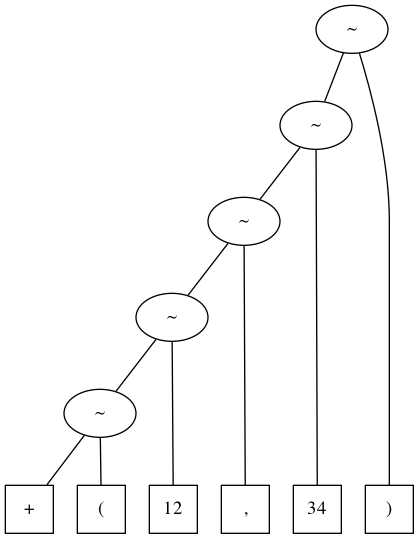
\includegraphics[width=.9\linewidth]{images/scala-parse-tree1.png}

For each token 
, 
, 
, 
, 
, 
, 
the binary operator  left-associatively created pairs.

But isn't it too complex? 
Because there are unnecessary tokens (, ,
). 
They consequently make the obtained syntax tree complex. 

The parser combinator of Scala has an operation which remove
unnecessary structures. 
So, there are two convenient operators: 
\begin{itemize}
\item If we use an operator  instead of 
    then the left hand side result is removed from the syntax tree.
\item In case we use  then the right hand side result is
removed from the syntax tree.
\end{itemize}

The following program \href{prog/parser/CalcP1.scala}{CalcP1.scala} removes unnecessary token from the
resulting syntax tree by using the operator . 
\begin{verbatim}
import scala.util.parsing.combinator._

object CalcP1 extends JavaTokenParsers {
  def expr: Parser[Any] = integer | (func <~ "(") ~ (expr <~ ",") ~ (expr <~ ")")
  def func = "+" | "-" | "*" | "/"
  def integer = wholeNumber
}
\end{verbatim}

We can execute it as follows. 
\begin{verbatim}
$ scala
scala> :load CalcP1.scala
scala> import CalcP1._
scala> parseAll(expr, "+(12,34)")
res: CalcP1.ParseResult[Any] = [1.9] parsed: ((+~12)~34)
\end{verbatim}

The obtained result represents the following syntax tree. 

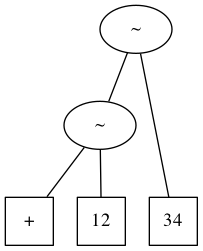
\includegraphics[width=.9\linewidth]{images/scala-parse-tree2.png}

\subsection{Exercise}
\label{sec:orgheadline6}
\begin{enumerate}
\item Modify CalcP1.scala to be able to use floating point numbers instead of integers. 
\begin{description}
\item[{}] For instance we can modify it as follows (\href{prog/parser/CalcP1float.scala}{CalcP1float.scala}).
\begin{verbatim}
def expr: Parser[Any] = 
          number | 
          (func <~ "(") ~ (expr <~ ",") ~ (expr <~ ")")
def func = "+" | "-" | "*" | "/"
def number = floatingPointNumber
\end{verbatim}
\end{description}
\item Modify CalcP1.scala to be able to use one argument operation/function like ``-(12)''= or =``abs(-34)''=. 
\begin{description}
\item[{}] For instance we can modify it as follows (\href{prog/parser/CalcP1unary.scala}{CalcP1unary.scala}). 
\begin{verbatim}
def expr: Parser[Any] =
  integer |
  (func1 <~ "(") ~ (expr <~ ")") |
  (func2 <~ "(") ~ (expr <~ ",") ~ (expr <~ ")")
def func1 = "-" | ident
def func2 = "+" | "-" | "*" | "/" | ident
def integer = wholeNumber
\end{verbatim}
Here, since we allow \texttt{ident} as the name of one argument
function name, we can use not only \texttt{abs} but also any
indentifiers. And, we can also use any two arguments function
names.
\end{description}
\item By using the following function \texttt{hexnum}, we can use integers of
Hexadecimal notation like \texttt{\#7E2} as tokens. 
\begin{verbatim}
def hexnum = "#" ~> "[0-9a-fA-F]+".r
\end{verbatim}
Modify CalcP1.scala to be able to use integers of Hexadecimal notations.
\begin{description}
\item[{}] For instance we can modify it like \href{prog/parser/CalcP1hex.scala}{CalcP1hex.scala}. 
\begin{verbatim}
import scala.util.parsing.combinator._

object CalcP1hex extends JavaTokenParsers {
  def expr: Parser[Any] =
    integer |
    hexnum |
    (func <~ "(") ~ (expr <~ ",") ~ (expr <~ ")")
  def func = "+" | "-" | "*" | "/"
  def integer = wholeNumber
  def hexnum = "#" ~> "[0-9a-fA-F]+".r
}
\end{verbatim}
\end{description}
\end{enumerate}

\subsection{Use of the result of parsing}
\label{sec:orgheadline7}
So far, we implemented a parser for formulas of prefix notations. 
The parse combinator of Scala allow us to describe any process we want 
after parsing. 
From here, let's implement a calculator by using this functionality. 
Note that, here, we assume results of calculation are integers. 
Calculators on floating point numbers will be an exercise lator.

How is the definition of expr in \href{prog/parser/CalcP1.scala}{CalcP1.scala} ?
It is given as follows. 
\begin{verbatim}
def expr: Parser[Any] = integer | (func <~ "(") ~ (expr <~ ",") ~ (expr <~ ")")
\end{verbatim}
\begin{verbatim}
def FunctionName: Parser[Any] = 
  Syntax Definition 1 | 
  Syntax Definition 2 | 
  ... | 
  Syntax Definition n
\end{verbatim}

In order to modify it to be able to return , a data
type of integers in Scala, we need to describe the followings. 
\begin{verbatim}
def FunctionName: Parser[Int] =
  Syntax Definition 1 ^^ Function 1 returning Int |
  Syntax Definition 2 ^^ Function 2 returning Int |
  ...
  Syntax Definition n ^^ Function n returning Int |
\end{verbatim}

Here, ``'' 
means a function which has 
\begin{itemize}
\item the results of parsing ``'' as input arguments and
\item return the result of calculation as  type.
\end{itemize}

``'' of expr is \texttt{integer}, and it returns
a string sequence as a result of parsing. 
So, the remaining task for ``'' 
is to implement a function which has a string 
representation of decimal integers as input arguments and returns a
Int value from it (data type is \texttt{String => Int}). 

By using anonymous functions of Scala, 
the function converting a string representation of decimal integers to
its value would be the followings:
\begin{itemize}
\item \texttt{(s => s.toInt)}
\item \texttt{\{ s => s.toInt \}}
\item \texttt{(\_.toInt)}
\item \texttt{\{ \_.toInt \}}
\end{itemize}
That is, we can write it as follows. 
\begin{verbatim}
def expr: Parser[Int] =
  integer ^^ { _.toInt } |
  (func <~ "(") ~ (expr <~ ",") ~ (expr <~ ")") ^^ { t => ... }
\end{verbatim}

``Syntax Definition 2'' of expr is \texttt{(func <\textasciitilde{} "(") \textasciitilde{} (expr <\textasciitilde{} ",") \textasciitilde{} (expr <\textasciitilde{} ")")} 
and it returns a structure like \texttt{(("+" \textasciitilde{} 12) \textasciitilde{} 34)} whose data type is \texttt{\textasciitilde{}[\textasciitilde{}[String,Int],Int]}.
The first element of this data structure  \texttt{(x \textasciitilde{} y)} is obtained by the
method  \texttt{.\_1} and similarly its second element is obtained by the method
\texttt{.\_2}. That is, if the value of \texttt{t} is \texttt{(("+" \textasciitilde{} 12) \textasciitilde{} 34)}, 
then we can obtain 12 by  \texttt{t.\_1.\_2} and obtain 34 by \texttt{t.\_2}.

In such a complex case, we can use ``switch expression'' of Scala.
\begin{verbatim}
t match {
  case pattern 1 => process 1
  case pattern 2 => process 2
  ...
  case pattern n => process n
}
\end{verbatim}

In this example, pattern matching of the structure of \texttt{t} is executed
from pattern 1, and process i is executed for the first pattern i
matched to the structure of \texttt{t}. 

A pattern for ``Syntax Definition 2'' of expr \texttt{(func <\textasciitilde{} "(") \textasciitilde{} (expr <\textasciitilde{}
",") \textasciitilde{} (expr <\textasciitilde{} ")")} can be written as \texttt{f \textasciitilde{} x \textasciitilde{} y}. 
Then, we can write it as follows.
\begin{verbatim}
def expr: Parser[Int] =
  integer ^^ { _.toInt } |
  (func <~ "(") ~ (expr <~ ",") ~ (expr <~ ")") ^^ { t => t match {
    case f ~ x ~ y => ...
  }}
\end{verbatim}

The part of \texttt{func} in the syntax definition is assigned to a variable \texttt{f}, 
First part of \texttt{expr} is assigned to a variable \texttt{x}, 
Next part of \texttt{expr} is assigned to a variable \texttt{y}. 
Note that, the data type of \texttt{f} is \texttt{String}, the data type of \texttt{x} and
\texttt{y} are \texttt{Int}. 

The value assigned to \texttt{f} is either =``+''=, =``-''=, =``*''=, or =``/''=.
So, for readability, we can write 4 patterns as follows.
\begin{verbatim}
def expr: Parser[Int] =
  integer ^^ { _.toInt } |
  (func <~ "(") ~ (expr <~ ",") ~ (expr <~ ")") ^^ { t => t match {
    case "+" ~ x ~ y => ...
    case "-" ~ x ~ y => ...
    case "*" ~ x ~ y => ...
    case "/" ~ x ~ y => ...
  }}
\end{verbatim}

In addition, we can write \texttt{\{ t => t match \{ ... \} \}} as simply \texttt{\{ ... \}}.
\begin{verbatim}
def expr: Parser[Int] =
  integer ^^ { _.toInt } |
  (func <~ "(") ~ (expr <~ ",") ~ (expr <~ ")") ^^ {
    case "+" ~ x ~ y => ...
    case "-" ~ x ~ y => ...
    case "*" ~ x ~ y => ...
    case "/" ~ x ~ y => ...
  }
\end{verbatim}

The following program is obtaned after we add process of calculating
values for each arithmetic operations. 
(\href{prog/parser/CalcP2.scala}{CalcP2.scala}).

\begin{verbatim}
import scala.util.parsing.combinator._

object CalcP2 extends JavaTokenParsers {
  def expr: Parser[Int] =
    integer ^^ { _.toInt } |
    (func <~ "(") ~ (expr <~ ",") ~ (expr <~ ")") ^^ {
      case "+" ~ x ~ y => x + y
      case "-" ~ x ~ y => x - y
      case "*" ~ x ~ y => x * y
      case "/" ~ x ~ y => x / y
    }
  def func = "+" | "-" | "*" | "/"
  def integer = wholeNumber
}
\end{verbatim}

The following is an example of execution.
\begin{verbatim}
scala> :load CalcP2.scala
scala> import CalcP2._
scala> parseAll(expr, "+(*(1,2), *(3,4))")
res: CalcP2.ParseResult[Int] = [1.18] parsed: 14
\end{verbatim}

\subsection{Exercise}
\label{sec:orgheadline8}
\begin{enumerate}
\item Modify CalcP2.scala to be able to use floating point numbers
instead of integers. Note that the data type of the result
becomes \texttt{Double}. 
\begin{description}
\item[{}] For instance, we can modify it like \href{prog/parser/CalcP2float.scala}{CalcP2float.scala}.
\end{description}
\item Further modify CalcP2.scala to be able to use more operations
like =``-(0.1)''=, =``abs(-2.3)''=, =``max(4, 5)''= . Note that we
assume that those process can be implemented as \texttt{math.abs(-2.3)},
\texttt{math.max((4, 5)}. Refer \href{http://www.scala-lang.org/api/current/scala/math/}{scala.math} package to check available
functions. 
\begin{description}
\item[{}] For instance, we can modify it like \href{prog/parser/CalcP2float2.scala}{CalcP2float2.scala}.
\end{description}
\end{enumerate}

\subsection{Extension to multiple arguments.}
\label{sec:orgheadline9}
Let's extend current program to allow multiple arguments like 
 (n \(\ge\) 1). 
This syntax can be defined by EBNF as follows. 
\begin{align*}
  \textit{expr} & ::=\ 
  \textit{integer}\ \mid\ 
  \textit{func}\ \mbox{"("}\ \textit{expr}\ \{\ \mbox{","}\ \textit{expr}\ \}\ \mbox{")"}
\end{align*}
Here, \(\{\ \alpha\ \}\) represents \(n\) time iterations of \(\alpha\) (\(n \ge 0\)).

Using the parser combinator of Scala, it can be written as follows. 
(\href{prog/parser/CalcP3.scala}{CalcP3.scala}).

\begin{verbatim}
import scala.util.parsing.combinator._

object CalcP3 extends JavaTokenParsers {
  def expr: Parser[Any] =
    integer |
    (func <~ "(") ~ expr ~ (rep("," ~> expr) <~ ")")
  def func = "+" | "-" | "*" | "/" | ident
  def integer = wholeNumber
}
\end{verbatim}

\texttt{rep("," \textasciitilde{}> expr)} corresponds to \(\{\ \mbox{","}\ \textit{expr}\ \}\)
Also, we add \texttt{ident} to the definition of \texttt{func} to be able to use any
identifiers as function names. 

We obtain the following results by running this program for \texttt{+(1,2,3,4)}.
\begin{verbatim}
scala> :load CalcP3.scala
scala> import CalcP3._
scala> parseAll(expr, "+(1,2,3,4)")
res: CalcP3.ParseResult[Any] = [1.11] parsed: ((+~1)~List(2, 3, 4))
\end{verbatim}

We can see that the result for the part of \texttt{rep("," \textasciitilde{}> expr)} becomes
a list of integers  \texttt{List(2,3,4)}. 
So, we can write the program for calculating the result of integers as follows.
\begin{verbatim}
def expr: Parser[Int] =
  integer ^^ { _.toInt } |
  (func <~ "(") ~ expr ~ (rep("," ~> expr) <~ ")") ^^ {
    case "+" ~ x ~ ys => ...
    case "-" ~ x ~ ys => ...
    case "*" ~ x ~ ys => ...
    case "/" ~ x ~ ys => ...
  }
\end{verbatim}

In case of \texttt{+(1,2,3,4)}, 
an integer \texttt{1} is assigned to a variable \texttt{x},
a list of integers \texttt{List(2,3,4)} is assigned to a variable \texttt{ys}.
So, we can calculate the result by \texttt{x + ys.sum} (\texttt{(x +: ys).sum} is
also fine). 

In case of \texttt{-(1,2,3,4)}, representing \(1-2-3-4\), 
the result is calculated as \texttt{x - ys.sum}. 
In case of \texttt{*(1,2,3,4)}, representing \(1\times 2\times 3\times 4\), 
the result is calculated as \texttt{x * ys.product}.
Similarly, \texttt{/(1,2,3,4)} is calculated as \texttt{x / ys.product}.

However, a problem will happen when we have only one argument.
The results of \texttt{+(1)}, \texttt{-(1)}, \texttt{*(1)}, \texttt{/(1)} are all \texttt{1}.
It is fine for \texttt{+}, \texttt{*}, \texttt{/} but \texttt{-1} should be returned in case \texttt{-(1)}.

It is resolved by writing a program as follows. 
(\href{prog/parser/CalcP4.scala}{CalcP4.scala}).

\begin{verbatim}
import scala.util.parsing.combinator._

object CalcP4 extends JavaTokenParsers {
  def expr: Parser[Int] =
    integer ^^ { _.toInt } |
    (func <~ "(") ~ expr ~ (rep("," ~> expr) <~ ")") ^^ {
      case "+" ~ x ~ ys => x + ys.sum
      case "-" ~ x ~ Nil => - x
      case "-" ~ x ~ ys => x - ys.sum
      case "*" ~ x ~ ys => x * ys.product
      case "/" ~ x ~ ys => x / ys.product
    }
  def func = "+" | "-" | "*" | "/" | ident
  def integer = wholeNumber
}
\end{verbatim}

In the program, a case pattern that will match when the part of \texttt{ys} is \texttt{Nil}.

\subsection{Exercise}
\label{sec:orgheadline10}
\begin{enumerate}
\item What is happen when we run CalcP4.scala with \texttt{parseAll(expr, "abs(-1)")} ?
\begin{description}
\item[{}] Parising goes well but we will have  \texttt{scala.MatchError} while
calculation because there is no pattern matched to \texttt{abs(x)}.
\end{description}
\item Modify CalcP4.scala to be able to use \texttt{abs(x)} which returns the
absolute value of \texttt{x}. 
\begin{description}
\item[{}] We can do that by adding the following line. 
\begin{verbatim}
case "abs" ~ x ~ Nil => math.abs(x)
\end{verbatim}
\end{description}
\item Modify CalcP4.scala to be able to get the result as \texttt{BigInt}
instead of \texttt{Int}. In addition, implement \texttt{fact(x)} which returns
the factorial of \texttt{x}. Note that we can translate a string \texttt{s} 
representing a decimal by using  \texttt{BigInt(s)}. 
\begin{description}
\item[{}] For instance, we can modify it as \href{prog/parser/CalcP4bigint.scala}{CalcP4bigint.scala}.
\end{description}
\end{enumerate}

\section{Special Exercise}
\label{sec:orgheadline13}
Modify \href{prog/parser/Work1.scala}{Work1.scala} to be able to do the followings. 

\begin{enumerate}
\item Add a function  \texttt{max(x1, x2, ..., xn)} which returns the maximum
value among x1, x2, \ldots{}, xn. 
\begin{description}
\item[{}] We can compute the maximum value of a list \texttt{ys} of \texttt{BigInt} by
using \texttt{ys.max}.
\end{description}
\item Add a function \texttt{gcd(x, y)} which returns the greatest common
devisor (GCD) for positive integers x and y. 
Refer \href{http://www.scala-lang.org/api/current/scala/math/BigInt.html}{scala.math.BigInt} for the calculatoin of the greatest common
devisor (GCD) for \texttt{BigInt}. 
\begin{description}
\item[{}] Use  \texttt{gcd} method of \texttt{BigInt}.
\end{description}
\item Add a function \texttt{gcd(x1, x2, ... xn)} which returns the greatest
common deviser (GCD) for positive integers x1, x2, \ldots{} xn. 
\begin{description}
\item[{}] Use \texttt{reduce} method for a list of  \texttt{BigInt}.
\end{description}
\item Add a function \texttt{lcm(x1, x2, ... xn)} which returns the least common
multiple (LCM) for positive integers  x1, x2, \ldots{} xn. 
\begin{description}
\item[{}] First, define a function \texttt{lcm(x, y)} which returns the least common
multiple for positive integer x and y as follows. Then, use
\texttt{reduce} for a given list x1, x2, \ldots{} xn. 
\begin{verbatim}
def lcm(x: BigInt, y: BigInt) = ...
\end{verbatim}
\end{description}
\end{enumerate}

\subsection{Verify}
\label{sec:orgheadline12}
Download \href{prog/parser/test1.txt}{test1.txt} to the same current directory. And run the programm
as follows. 

\begin{verbatim}
scala> :load Work1.scala
scala> Work1.test
\end{verbatim}

\begin{itemize}
\item \texttt{OK} denotes everything is fine!
\item \texttt{NG} denotes that parsing is fine but the calculation result is wrong.
\item \texttt{ERR} denotes that parsing is wrong.
\item \texttt{scala.MatchError} denotes your program is incorrect.
\end{itemize}
\end{document}
